% Section content template for individual Educative lessons
% This file contains the actual content for a specific section
% Generated from Educative API section content

% Section: Inheritance
% Section ID: 5510500085661696
% Section Slug: inheritance
% Generated: 2025-12-16T12:49:25.640801

\subsection{Definition}\label{a25MENAPZzo3HDXW8NUDX-1}
\\
\textbf{Inheritance}~provides a way to create a new class from an existing class. The new class is a specialized version of the existing class such that it inherits all the~public~attributes (variables) and~methods~of the existing class. The existing class is used as a starting point or base~to create the new class.

\subsection{The IS-A relationship}\label{VCprC7UIsg4i69Z0lB69-}
\\
After reading the definition above, the next question that comes to mind is, ``when do we use inheritance?'' Wherever we come across an~IS-A~relationship between objects, we can use inheritance.

\begin{figure}[htbp]
 \centering
 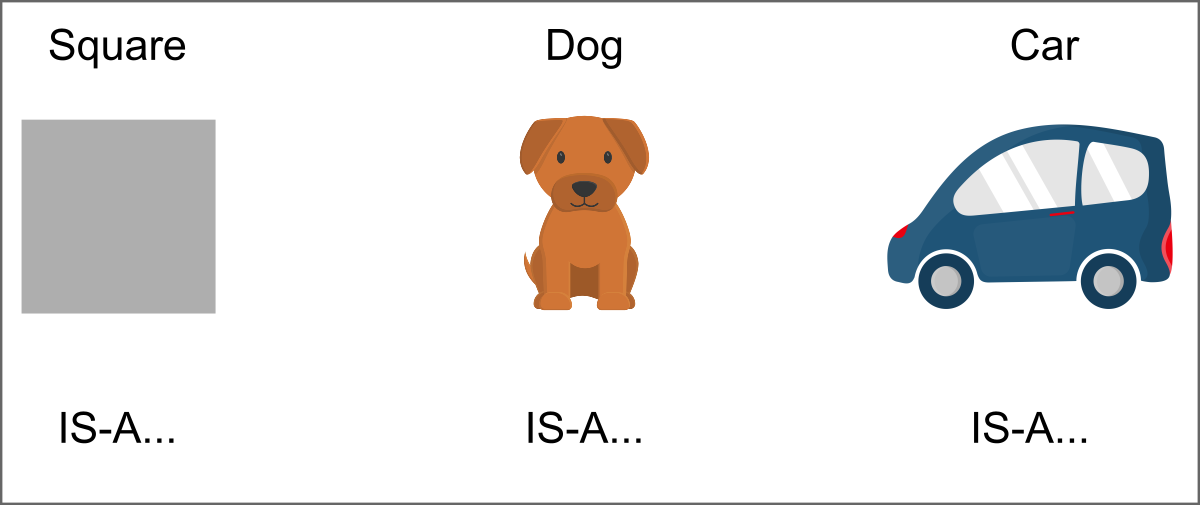
\includegraphics[width=0.5\textwidth]{Images/chapter_2/section_5510500085661696/6486587921924096.png}
 \caption{The IS-A relationship}
\end{figure}

So, from the description of inheritance above, we can conclude that we can build new classes by extending~existing classes.

\begin{table}[htbp]
\centering
\small
\adjustbox{max width=\textwidth}{
\begin{tabular}{|p{0.481\textwidth}|p{0.469\textwidth}|}
\hline
\textbf{Existing Class} & \textbf{Derived Class} \\
\hline
\hline
Shape \hfill\break Animal \hfill\break Vehicle & Square \hfill\break Dog \hfill\break Car \\
\hline
\hfill\break & \hfill\break \\
\hline
\hfill\break & \hfill\break \\
\hline
\end{tabular}
}
\end{table}

Let's look at the figure below to visualize some examples where an IS-A relationship doesn't exist.

\begin{figure}[htbp]
 \centering
 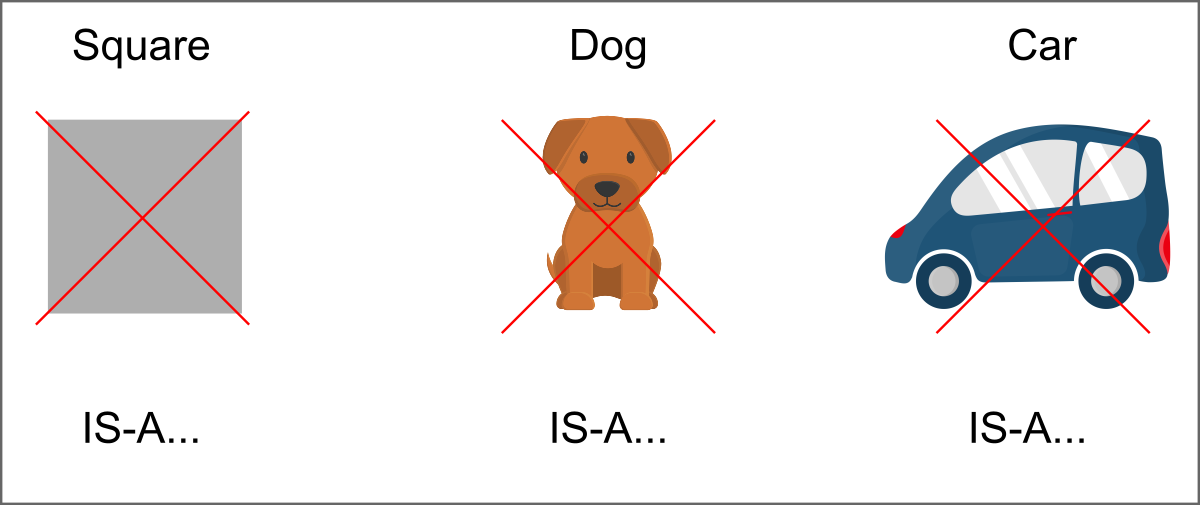
\includegraphics[width=0.5\textwidth]{Images/chapter_2/section_5510500085661696/4957877536292864.png}
 \caption{The IS-A relationship does not exist}
\end{figure}

Remember, we cannot use inheritance if an IS-A relationship doesn't exist between classes.

\subsection{Modes of inheritance}\label{9gK4Uuzx-tWVRm2CpJQkx}
\\
\textbf{Access modifiers} are tags we can associate with each member to define the parts of the program they can access directly. ~By using these modifiers, we define the scope of the data members and member functions for the other classes and main.

\subsection{Types of inheritance}\label{1YTq6oCywdYl8DkbSK9cu}
\\
Based on parent classes and child classes, there are \emph{five} types of inheritance in general, which are explained below.

\subsubsection{Single inheritance}\label{ajGSKYLn4RycF503L83lH}
\\
In single inheritance, there is only a single class extending from a single parent class.
\\
\textbf{Example:}

\begin{itemize}
\item
\protect\phantomsection\label{uXxme5r_vFyBXeOGsL4qm}
A fuel car IS-Avehicle
\end{itemize}

\begin{figure}[htbp]
 \centering
 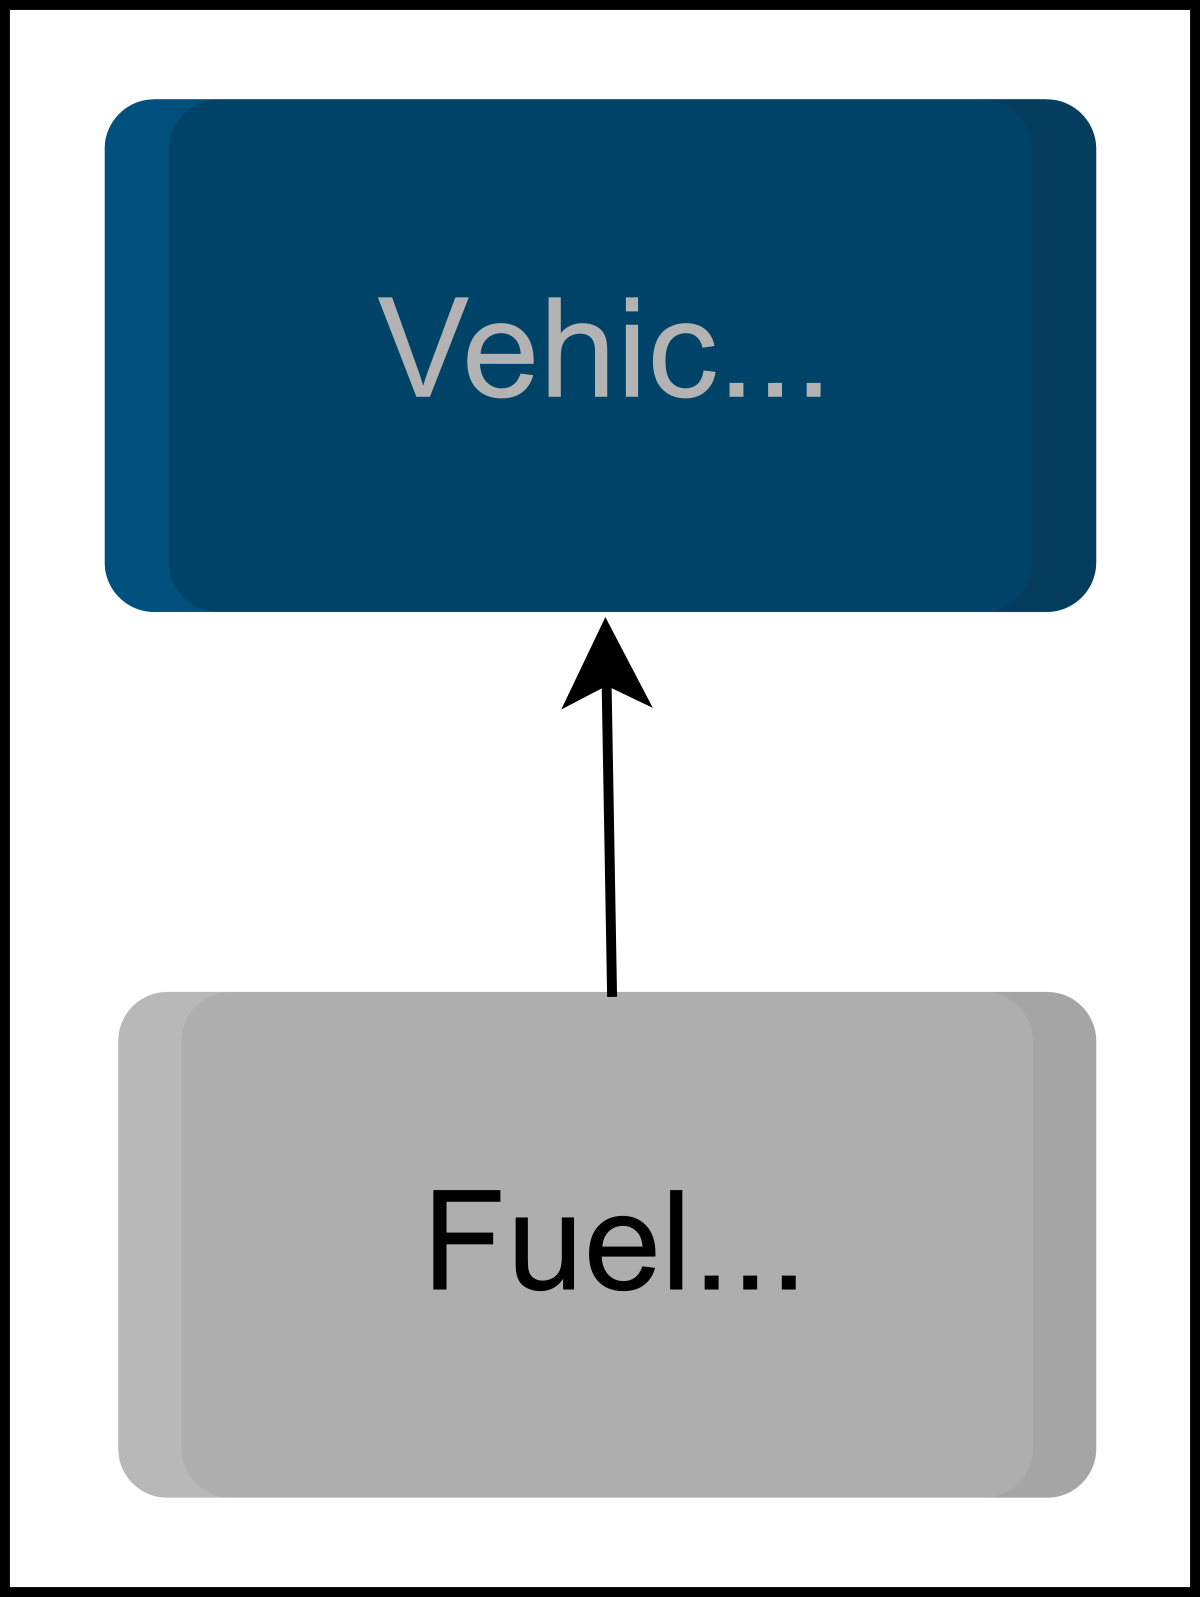
\includegraphics[width=0.5\textwidth]{Images/chapter_2/section_5510500085661696/5755299966484480.png}
 \caption{Single inheritance}
\end{figure}

\subsubsection{Multiple inheritance}\label{ltmb7HAfOPLmqpWBFxJto-1}
\\
When a class is derived from more than one base class, i.e., when a class has more than one immediate parent class, it is called multiple inheritance.
\\
\textbf{Example:}

\begin{itemize}
\item
\protect\phantomsection\label{P86rLdb6t0WPclm3KfUu2}
The hybrid car~IS-A~fuel car.
\item
\protect\phantomsection\label{NT1USYneSyyhEkMKvVxW0}
The hybrid car~IS-A~electric car~as well.
\end{itemize}

\begin{figure}[htbp]
 \centering
 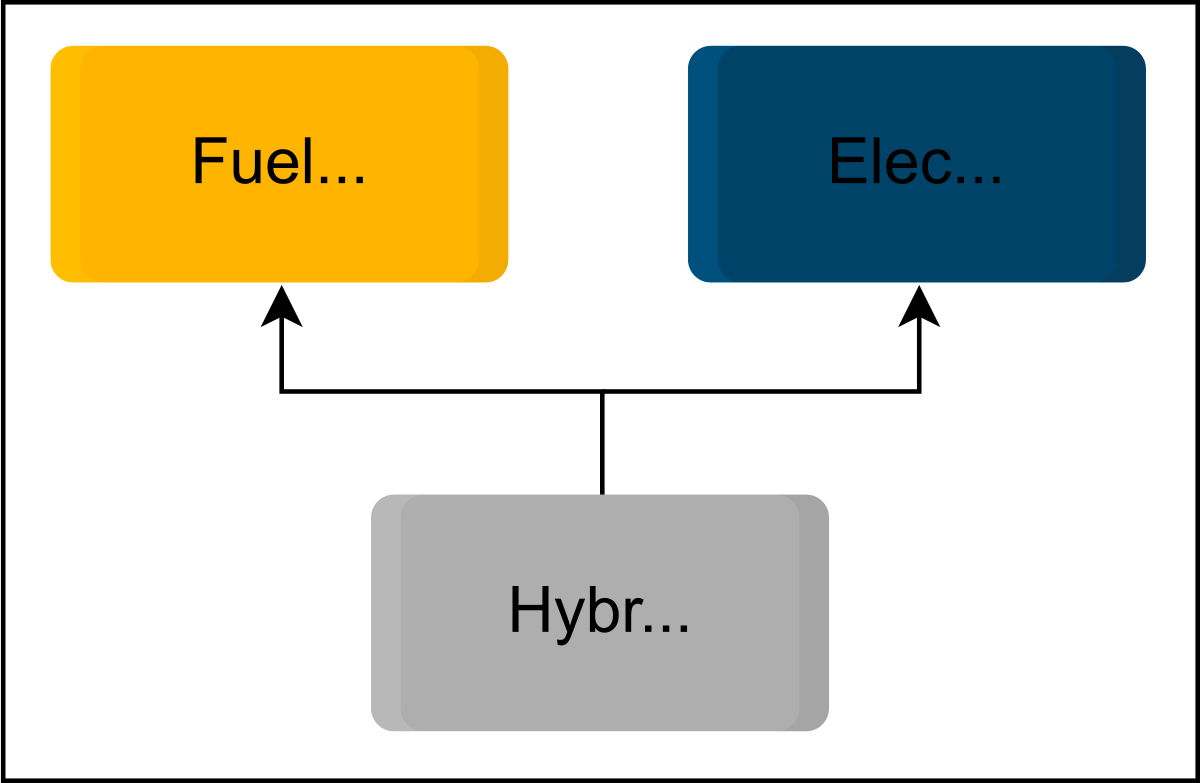
\includegraphics[width=0.5\textwidth]{Images/chapter_2/section_5510500085661696/6117249275658240.png}
 \caption{Multiple inheritance}
\end{figure}

\subsubsection{Multi-level inheritance}\label{ltmb7HAfOPLmqpWBFxJto-2}
\\
When a class is derived from a class that itself is derived from another class, it is called multi-level inheritance. We can extend the classes to as many levels as we want.
\\
\textbf{Example:}

\begin{itemize}
\item
\protect\phantomsection\label{LH0g2CDEidJxvbB5U6q7O}
A~fuel car~IS-A~vehicle
\item
\protect\phantomsection\label{aAhBFe-g5sRiBpIaPtMhC}
A~gasoline car~IS-A~fuel car
\end{itemize}

\begin{figure}[htbp]
 \centering
 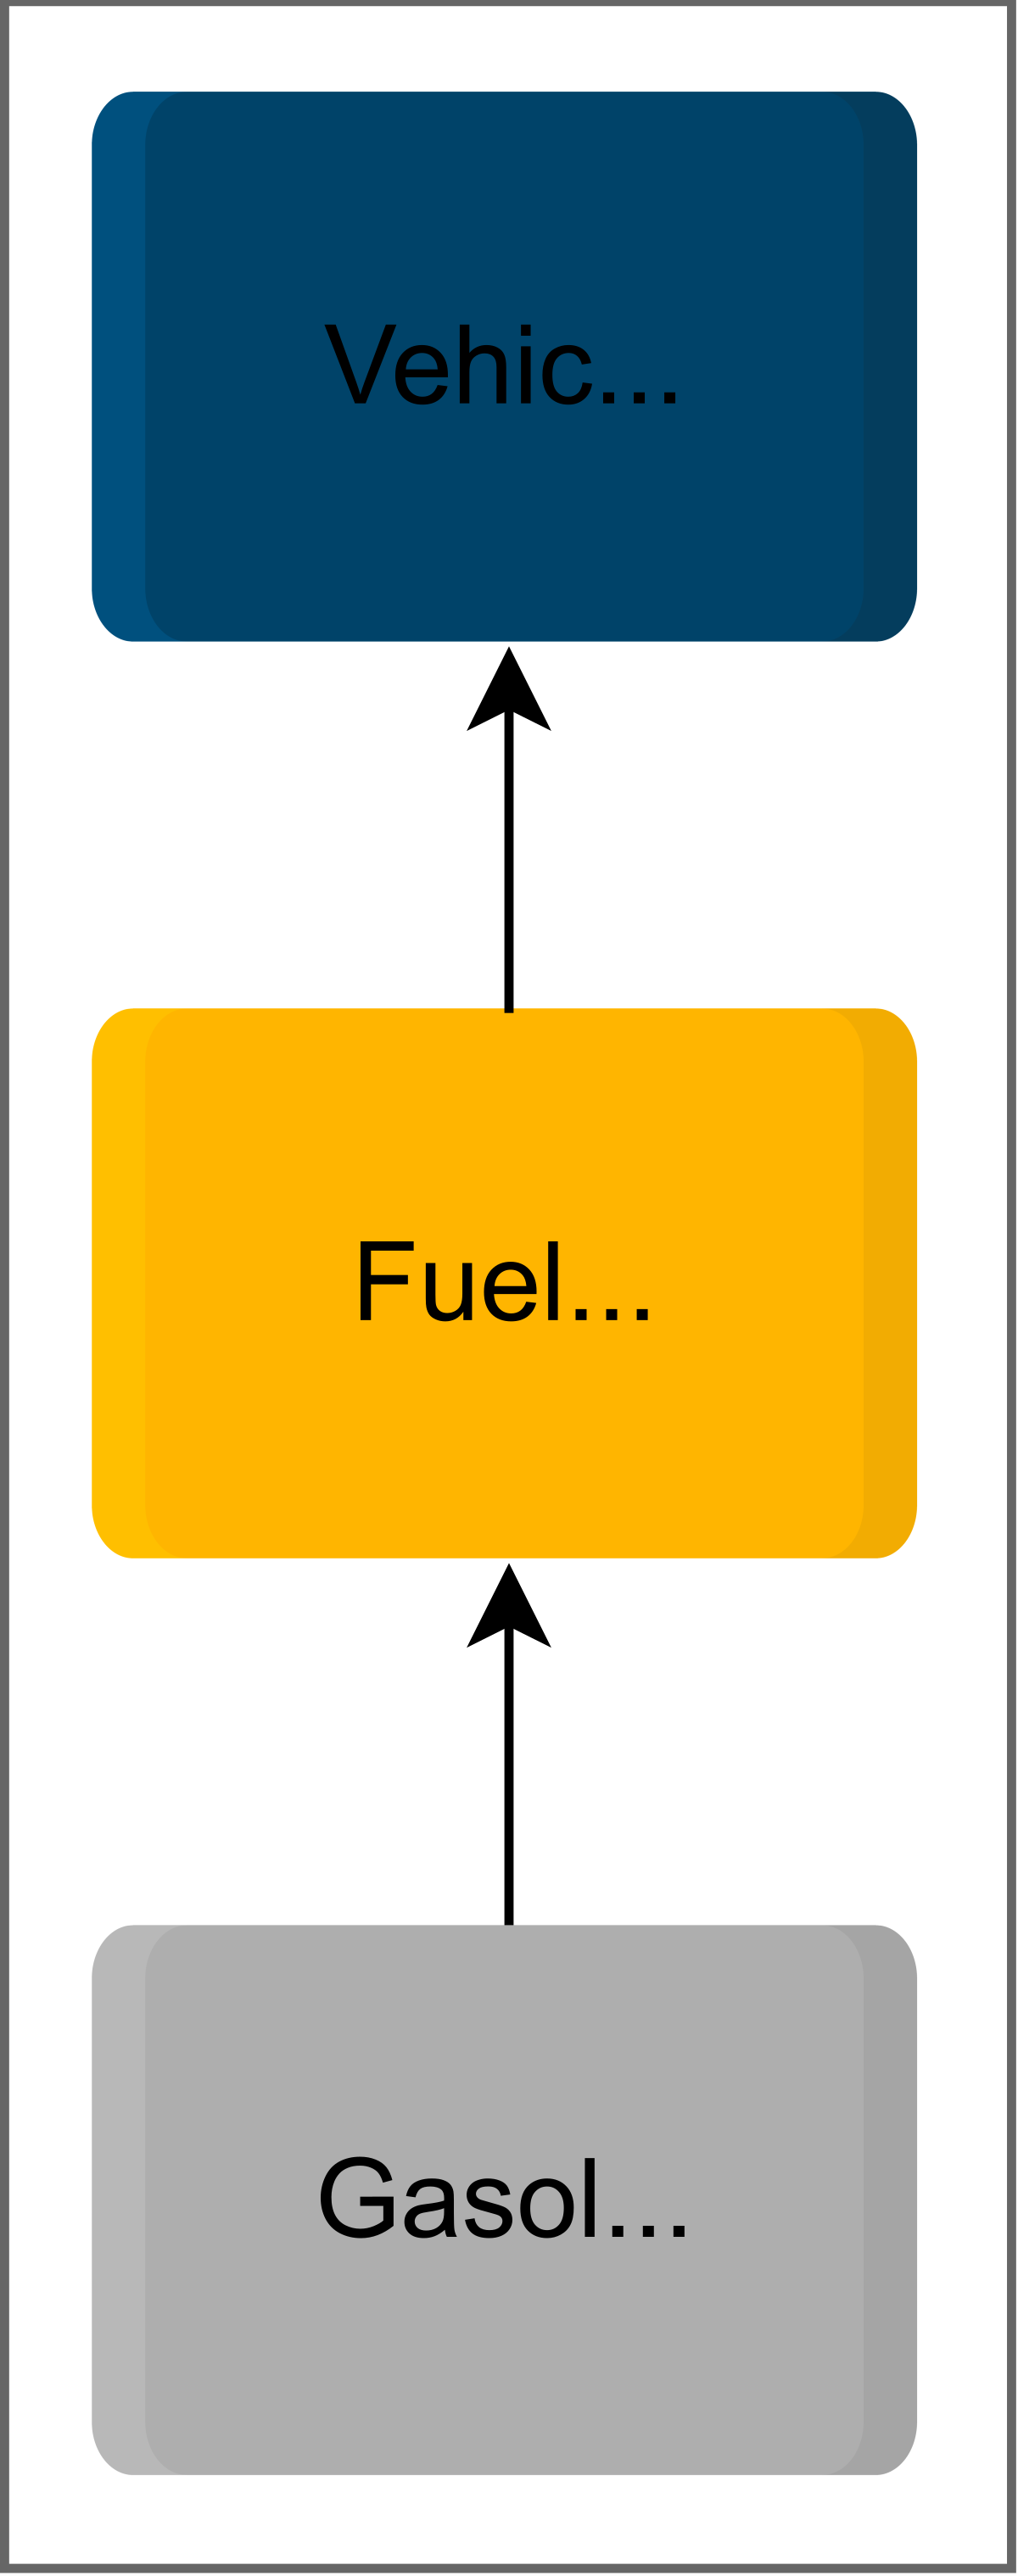
\includegraphics[width=0.5\textwidth]{Images/chapter_2/section_5510500085661696/5989506210856960.png}
 \caption{Multi-level inheritance}
\end{figure}

\subsubsection{Hierarchical inheritance}\label{ltmb7HAfOPLmqpWBFxJto-3}
\\
In hierarchical inheritance, more than one class extends, as per the requirement of the design, from the same base class. The common attributes of these child classes are implemented inside the base class.
\\
\textbf{Example:}

\begin{itemize}
\item
\protect\phantomsection\label{agkJ1L8CLRvNb4EbjCLMK}
A~fuel car~IS-A~vehicle
\item
\protect\phantomsection\label{50BhYToONZbdSiVr410dE}
An electric car~IS-A~vehicle
\end{itemize}

\begin{figure}[htbp]
 \centering
 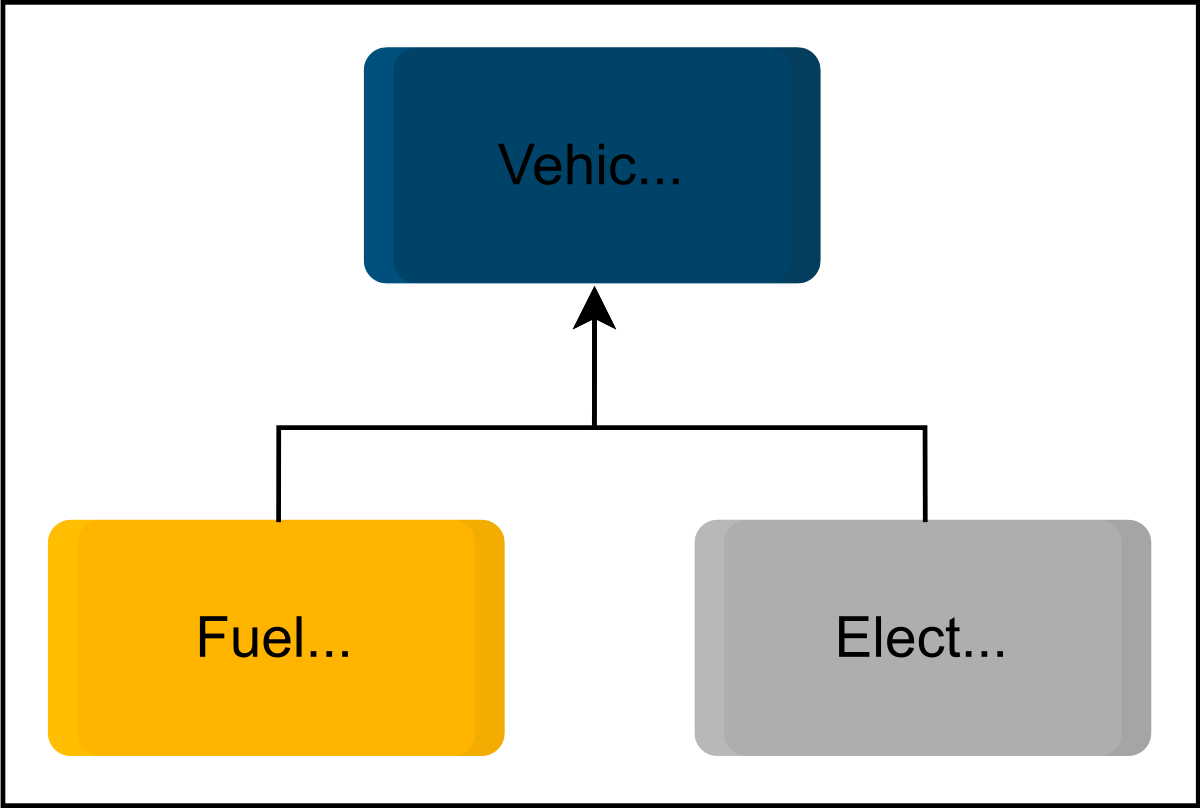
\includegraphics[width=0.5\textwidth]{Images/chapter_2/section_5510500085661696/6128065295155200.png}
 \caption{Hierarchical inheritance}
\end{figure}

\subsubsection{Hybrid inheritance}\label{ltmb7HAfOPLmqpWBFxJto-4}
\\
A type of inheritance that is a combination of more than one type of inheritance is called \textbf{hybrid inheritance}.
\\
\textbf{Example:}

\begin{itemize}
\item
\protect\phantomsection\label{AwT_w6Kf2B-reHfJgkX79}
A fuel car~IS-A~vehicle.
\item
\protect\phantomsection\label{nRWZy5j5z7TFPTSpBub2J}
An electric car~IS-A~vehicle.
\item
\protect\phantomsection\label{iPfmcFlnlR_-jUIYQWKzj}
A hybrid car~IS-A~fuel car~and IS-A~electric car.
\end{itemize}

\begin{figure}[htbp]
 \centering
 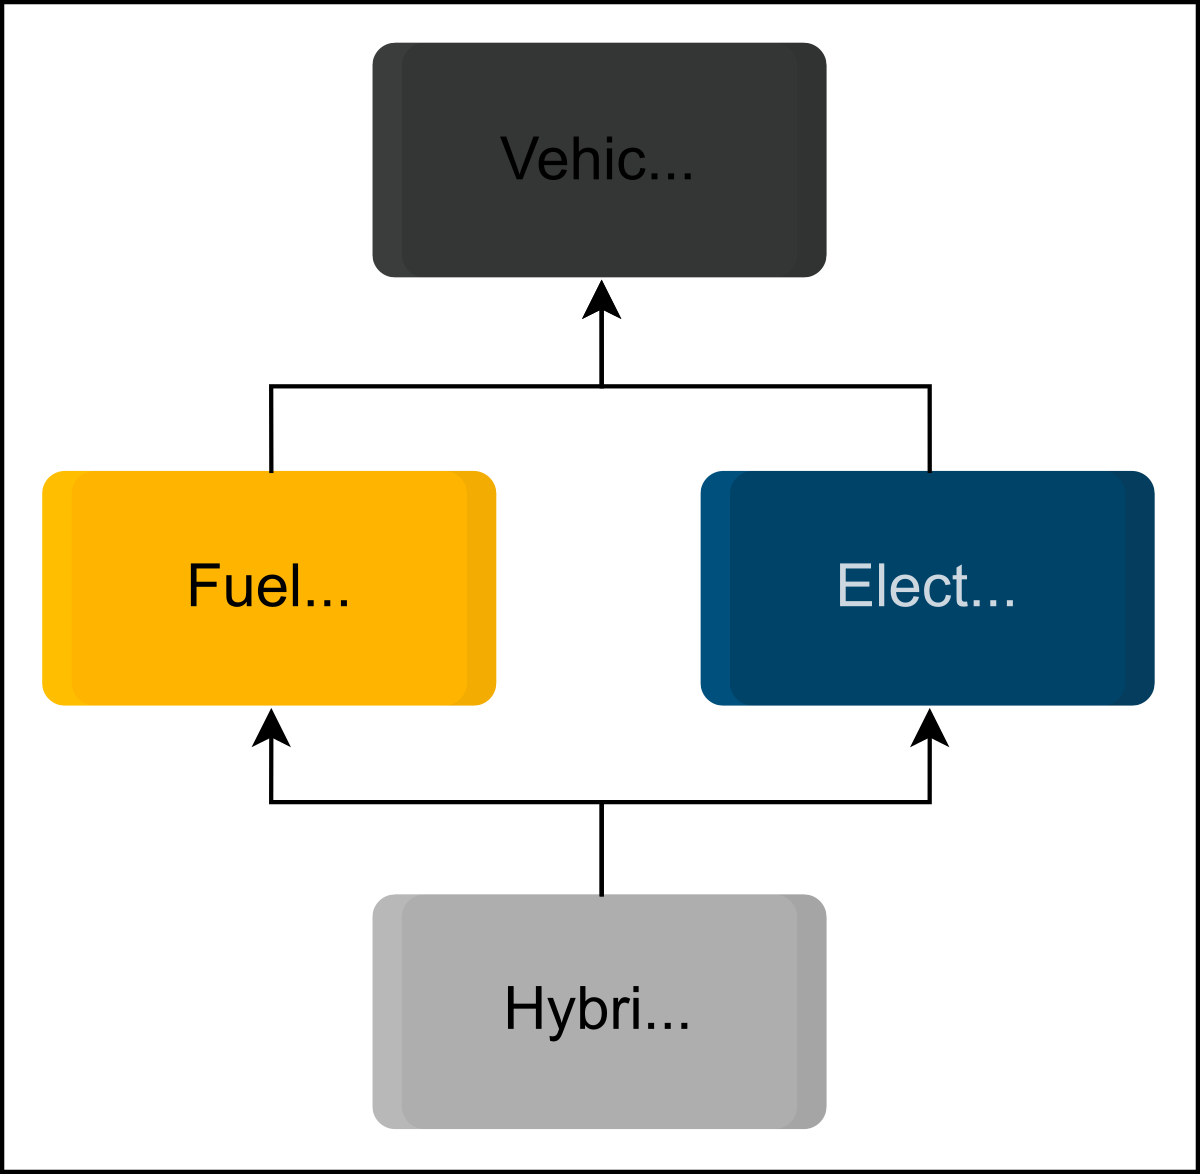
\includegraphics[width=0.5\textwidth]{Images/chapter_2/section_5510500085661696/6552069885657088.png}
 \caption{Hybrid inheritance}
\end{figure}

\subsection{Implementation}\label{6TKkViZvBQEXJXAQ7E7w--1}
\\
Let's take an example of a \texttt{Vehicle} class and implement different classes that will extend from it. We will also implement hierarchical, multi-level, and multiple inheritances from this example.
\begin{quote}
\textbf{Note:} Some languages, such as Java, C\# and JavaScript, do not support multiple inheritance through classes.
\end{quote}

\textbf{The implementation of various classes using inheritance}

\begin{lstlisting}[language=Java]
// Base class (Parent)

class Vehicle {

    private String name;

    private String model;

    Vehicle(String name, String model) {

        this.name = name;

        this.model = model;

    }

    public void getName() {

        System.out.print("The car is a " + name + " " + model);

    }

}



// Single inheritance

// FuelCar class extending from Vehicle class

// Derived class (Child)

class FuelCar extends Vehicle {

    private String combustType;

    FuelCar(String name, String model, String combustType) {

        super(name, model);

        this.combustType = combustType;

    }

    public void getFuelCar() {

        getName();

        System.out.print(", combust type is " + combustType);

    }

}



// Hierarchical inheritance

// Alongside the FuelCar class, the ElectricCar class is also extending from Vehicle class

// Another Derived class (Child)

class ElectricCar extends Vehicle {

    private String batteryPower;

    ElectricCar(String name, String model, String batteryPower) {

        super(name, model);

        this.batteryPower = batteryPower;

    }

    public void getElectricCar() {

        getName();

        System.out.print(", battery power is " + batteryPower);

    }

}



// Multi-level inheritance

// GasolineCar class is derived from the FuelCar class, which is further derived from the Vehicle class

// Derived class (Grandchild)

class GasolineCar extends FuelCar {

    private String combustType;

    private String gasCapacity;

    GasolineCar(String name, String model, String combustType, String gasCapacity) {

        super(name, model, combustType);

        this.gasCapacity = gasCapacity;

    }

    public void getGasolineCar() {

        getName();

        System.out.print(", gas capacity is " + gasCapacity);

    }

}



// Java does not support Multiple inheritance via classes



// main

public class main

{

    public static void main(String[] args) {

        System.out.println("Single inheritance:");

        FuelCar Fuel = new FuelCar("Honda", "Accord", "Petrol");

        Fuel.getFuelCar();

        System.out.println("
");



        System.out.println("Hierarchical inheritance:");

        ElectricCar Electric = new ElectricCar("Tesla", "ModelX", "200MWH");

        Electric.getElectricCar();

        System.out.println("
");



        System.out.println("Multi-Level inheritance:");

        GasolineCar Gasoline = new GasolineCar("Toyota", "Corolla", "Gasoline", "30 liters");

        Gasoline.getGasolineCar();

        

        

        System.out.println("
");

        System.out.println("Java does not support Multiple Inheritance through classes");

    }

}
\end{lstlisting}

\subsection{Advantages of inheritance}\label{6TKkViZvBQEXJXAQ7E7w--2}
\\
The following are four main advantages of inheritance:

\begin{table}[htbp]
\centering
\small
\adjustbox{max width=\textwidth}{
\begin{tabular}{|p{0.173\textwidth}|p{0.777\textwidth}|}
\hline
\textbf{Advantages} & \textbf{Description} \\
\hline
\hline
\hfill\break & \hfill\break \\
\hline
Reusability & We don't need to duplicate \textbf{} methods inside the child classes that also occur in the parent classes. \\
\hline
Code modification & Ensures that all changes are localized and inconsistencies are avoided. \\
\hline
Extensibility & We can extend the base class as per the requirements of the derived class. It provides an easy way to upgrade or enhance specific parts of a product without changing the core attributes. \\
\hline
Data hiding & A base class can keep some data private so that the derived class cannot alter it. This concept is called encapsulation. \\
\hline
\end{tabular}
}
\end{table}

Let\textquotesingle s learn about polymorphism in the next lesson.

% End of section content